\documentclass[11pt]{article}

% Packages shared by the whole paper. Keep document-specific macros in main.tex.
\usepackage[margin=1in]{geometry}
\usepackage{amsmath,amsfonts,amssymb,amsthm}
\usepackage{graphicx}
\graphicspath{{figures/}{../build/figures/}}
\usepackage{xcolor}
\usepackage{enumitem}
\usepackage{booktabs}
\usepackage{listings}

% Graphics. PSTricks needs the DVI -> PostScript route (see latexmkrc); TikZ
% works on either route.
\usepackage{pstricks}
\usepackage{pst-plot}
\usepackage{tikz}
\usetikzlibrary{arrows.meta,positioning,shapes,calc}

% hyperref last, cleveref after hyperref.
\usepackage[hidelinks]{hyperref}
\usepackage{cleveref}

\newtheorem{theorem}{Theorem}[section]
\newtheorem{definition}[theorem]{Definition}

% Palette for code listings and figures.
\definecolor{codegray}{gray}{0.9}
\definecolor{codebackground}{rgb}{0.97,0.97,0.97}
\definecolor{codeblue}{rgb}{0,0,0.6}
\definecolor{codegreen}{rgb}{0,0.5,0}
\definecolor{codepurple}{rgb}{0.58,0,0.82}
\definecolor{codeorange}{rgb}{0.85,0.45,0}
\definecolor{codered}{rgb}{0.8,0,0}
\definecolor{codeteal}{rgb}{0,0.5,0.5}

\definecolor{figprimary}{rgb}{0.16,0.45,0.85}
\definecolor{figaccent}{rgb}{0.95,0.55,0.15}
\definecolor{figmuted}{rgb}{0.6,0.6,0.6}

% Code listings. Uses `listings` (pure TeX, no shell-escape or Python needed).
% If you prefer Pygments highlighting, install `minted` in docker/Dockerfile
% (TLMGR_EXTRA="minted") and pass -shell-escape in latexmkrc.

\lstdefinelanguage{typescript}{
  keywords={abstract, as, async, await, break, case, catch, class, const,
    continue, debugger, default, delete, do, else, enum, export, extends,
    false, finally, for, from, function, if, implements, import, in,
    instanceof, interface, let, new, null, of, package, private, protected,
    public, readonly, return, static, super, switch, this, throw, true, try,
    type, typeof, undefined, var, void, while, with, yield},
  ndkeywords={boolean, number, string, any, never, unknown, object, symbol,
    bigint, Promise, Record, Partial, Array},
  sensitive=true,
  comment=[l]{//},
  morecomment=[s]{/*}{*/},
  morestring=[b]',
  morestring=[b]", % chktex 18
  morestring=[b]`
}

\lstdefinelanguage{sql-extended}[]{SQL}{
  morekeywords={POLICY, ROW, LEVEL, SECURITY, ENABLE, USING, RETURNS, LANGUAGE,
    BEGIN, END, DECLARE, IF, THEN, ELSE, LOOP, RAISE, EXCEPTION, STABLE,
    IMMUTABLE, VOLATILE, SECURITY, DEFINER, INVOKER, SETOF, TRIGGER, BEFORE,
    AFTER, EACH, EXECUTE, FUNCTION, PROCEDURE, REPLACE, CURRENT_SETTING},
  sensitive=false
}

\lstdefinestyle{paper}{
  backgroundcolor=\color{codebackground},
  basicstyle=\ttfamily\footnotesize,
  keywordstyle=\color{codeblue}\bfseries,
  ndkeywordstyle=\color{codeteal},
  commentstyle=\color{codegreen}\itshape,
  stringstyle=\color{codepurple},
  numberstyle=\tiny\color{figmuted},
  numbers=left,
  numbersep=8pt,
  frame=single,
  framerule=0pt,
  xleftmargin=1.5em,
  breaklines=true,
  breakatwhitespace=true,
  keepspaces=true,
  showstringspaces=false,
  tabsize=2,
  captionpos=b
}
\lstset{style=paper}


\title{____title____}
\author{____fullName____ \\ \texttt{____email____}}
\date{\today}

\begin{document}

\maketitle

\begin{abstract}
  This document was generated from the Mathapedia LaTeX boilerplate. It compiles
  with the classic \texttt{latex} $\rightarrow$ \texttt{dvips} $\rightarrow$
  \texttt{ps2pdf} pipeline so PSTricks and TikZ figures both work, and every
  figure in it is a text file, so the whole paper is diffable.
\end{abstract}

\tableofcontents

\section{Introduction}
\label{sec:introduction}

Replace this section with your own. The skeleton exercises everything the
build pipeline has to support so a broken toolchain shows up on the first
\texttt{make build}, not the week before a deadline: cross references
(\cref{sec:graphics}), citations~\cite{knuth1984texbook,vanzandt1993pstricks},
theorem environments, and both figure systems.

\begin{definition}[Paper]
  \label{def:paper}
  A \emph{paper} is a directory containing \texttt{tex/main.tex} such that
  \texttt{make build} produces \texttt{build/main.pdf}.
\end{definition}

\begin{theorem}
  \label{thm:reproducible}
  If every figure in a paper is a text file and the toolchain is pinned in
  \texttt{docker/Dockerfile}, then \cref{def:paper} holds on every machine with
  Docker installed.
\end{theorem}

\begin{proof}
  The TeX Live image is content addressed and the sources are in git;
  \texttt{latexmk} is deterministic given both. See
  \cref{sec:graphics,sec:code} for what ``figure'' and ``text file'' cover.
\end{proof}

Inline math renders as usual, $e^{i\pi} + 1 = 0$, as does display math:
\begin{equation}
  \label{eq:gauss}
  \int_{-\infty}^{\infty} e^{-x^2}\,\mathrm{d}x = \sqrt{\pi}.
\end{equation}

\section{Graphics}
\label{sec:graphics}

Three kinds of figure are supported, and they have different rendering
stories, so pick deliberately:

\begin{itemize}[nosep]
  \item \textbf{PSTricks} (\cref{fig:pie,fig:plot}) --- rendered by
    \texttt{dvips}/Ghostscript in the PDF build. The subset used here
    (\texttt{pspicture}, \texttt{psline}, \texttt{pscircle}, \texttt{pswedge},
    \texttt{psplot}, \texttt{psaxes}, \texttt{rput}, \texttt{psdots}) is also
    what LaTeX2JS renders in the browser, so these figures can be reused as-is
    on Mathapedia.
  \item \textbf{TikZ} (\cref{fig:flow}) --- rendered in the PDF build only.
    Use it for diagrams that will never need a browser rendering.
  \item \textbf{Generated EPS} (\cref{fig:pipeline}) --- anything produced by an
    external tool (Mermaid here). \texttt{make figures} turns
    \texttt{tex/figures/*.mmd} into \texttt{build/figures/*.eps}; only the
    source is committed.
\end{itemize}

\begin{figure}[ht]
  \centering
  % PSTricks: circle, wedges, labels, arrows. Stays inside the LaTeX2JS subset
% so the same source renders on Mathapedia. Keep PSTricks commands at column
% 0 inside pspicture: the browser parser does not tolerate leading whitespace.
\begin{pspicture}(-3.5,-3.5)(5,3.5)
\pscircle[linewidth=0.5pt](0,0){3}
\pswedge[fillstyle=solid,fillcolor=figaccent,linestyle=none](0,0){3}{60}{120}
\pswedge[fillstyle=solid,fillcolor=figprimary,linestyle=none](0,0){3}{120}{420}
\rput(4,2.5){\textbf{one sixth}}
\psline{->}(3.2,2.3)(0.3,2.3)
\rput(-2.6,-2.8){\textbf{five sixths}}
\psline{->}(-2.4,-2.4)(-1.3,-1.3)
\psdots[dotstyle=o,dotsize=3pt](0,0)
\end{pspicture}

  \caption{A PSTricks figure. Everything in it is in the LaTeX2JS subset.}
  \label{fig:pie}
\end{figure}

\begin{figure}[ht]
  \centering
  % PSTricks plot (pst-plot). psaxes + psplot are in the LaTeX2JS subset.
\begin{pspicture}(-0.5,-1.5)(6.5,1.7)
\psaxes[labels=none,ticks=none]{->}(0,0)(-0.5,-1.5)(6.5,1.5)
\psplot[linecolor=figprimary,linewidth=1.2pt,plotpoints=200]{0}{6.28}{x 57.2958 mul sin}
\psplot[linecolor=figaccent,linewidth=1.2pt,plotpoints=200]{0}{6.28}{x 57.2958 mul cos}
\rput(6.5,-0.3){$x$}
\rput(-0.3,1.5){$y$}
\rput(3.2,1.4){\color{figprimary}$\sin x$}
\rput(1.4,-1.3){\color{figaccent}$\cos x$}
\end{pspicture}

  \caption{A PSTricks plot with axes; \texttt{psplot} is interactive on Mathapedia.}
  \label{fig:plot}
\end{figure}

\begin{figure}[ht]
  \centering
  % TikZ: the build pipeline as a flow diagram. PDF only (no browser rendering).
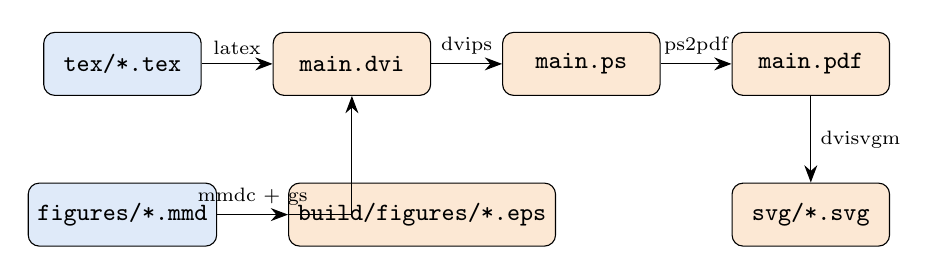
\begin{tikzpicture}[
  node distance=1.1cm and 0.9cm,
  box/.style={draw,rounded corners,minimum width=2cm,minimum height=0.8cm,
              align=center,font=\small},
  src/.style={box,fill=figprimary!15},
  art/.style={box,fill=figaccent!20},
  >={Stealth[length=2.2mm]}
]
\node[src] (tex) {\texttt{tex/*.tex}};
\node[src,below=of tex] (mmd) {\texttt{figures/*.mmd}};
\node[art,right=of mmd] (eps) {\texttt{build/figures/*.eps}};
\node[art,right=of tex] (dvi) {\texttt{main.dvi}};
\node[art,right=of dvi] (ps) {\texttt{main.ps}};
\node[art,right=of ps] (pdf) {\texttt{main.pdf}};
\node[art,below=of pdf] (svg) {\texttt{svg/*.svg}};

\draw[->] (tex) -- node[above,font=\scriptsize] {latex} (dvi);
\draw[->] (dvi) -- node[above,font=\scriptsize] {dvips} (ps);
\draw[->] (ps) -- node[above,font=\scriptsize] {ps2pdf} (pdf);
\draw[->] (mmd) -- node[above,font=\scriptsize] {mmdc + gs} (eps);
\draw[->] (eps) -| (dvi);
\draw[->] (pdf) -- node[right,font=\scriptsize] {dvisvgm} (svg);
\end{tikzpicture}

  \caption{A TikZ figure. PDF only.}
  \label{fig:flow}
\end{figure}

\begin{figure}[ht]
  \centering
  \includegraphics[width=0.85\linewidth]{pipeline}
  \caption{A Mermaid diagram compiled to EPS by \texttt{make figures}.}
  \label{fig:pipeline}
\end{figure}

\section{Code}
\label{sec:code}

Listings use the \texttt{listings} package with the languages defined in
\texttt{tex/headers/listings.tex}. \Cref{lst:ts} is TypeScript,
\cref{lst:sql} is SQL with the PL/pgSQL and RLS keywords added.

\begin{lstlisting}[language=typescript,caption={A TypeScript listing.},label={lst:ts}]
export interface Paper {
  title: string;
  authors: readonly string[];
}

export async function build(paper: Paper): Promise<Uint8Array> {
  const pdf = await latexmk(paper, { mode: 'pdfps' });
  return pdf; // generics like Map<string, Paper> render fine
}
\end{lstlisting}

\begin{lstlisting}[language=sql-extended,caption={A SQL listing.},label={lst:sql}]
CREATE POLICY papers_owner ON papers
  FOR SELECT
  USING (owner_id = current_setting('jwt.claims.user_id', true)::uuid);

ALTER TABLE papers ENABLE ROW LEVEL SECURITY;
\end{lstlisting}


\bibliographystyle{IEEEtran}
\bibliography{references}

\end{document}
